%Este trabalho está licenciado sob a Licença Creative Commons Atribuição-CompartilhaIgual 3.0 Não Adaptada. Para ver uma cópia desta licença, visite http://creativecommons.org/licenses/by-sa/3.0/ ou envie uma carta para Creative Commons, PO Box 1866, Mountain View, CA 94042, USA.

%\documentclass[main.tex]{subfiles}
%\begin{document}

\chapter{Problemas de valores de contorno}\index{Problemas de valores de contorno}

Neste capítulo, tratamos dos métodos numéricos para resolver equações diferenciais ordinárias com condições de contorno.

%%%%%%%%%%%%%%%%%%%%
% python
\ifispython
Nos códigos \verb+Python+ apresentados, assumimos que as seguintes bibliotecas e módulos estão carregados:
\begin{verbatim}
>>> from __future__ import division
>>> import numpy as np
>>> from numpy import linalg
>>> import matplotlib.pyplot as plt
\end{verbatim}
\fi
%%%%%%%%%%%%%%%%%%%%

\section{Método de diferenças finitas}

Nesta seção, discutimos os fundamentos do \emph{método de diferenças finitas}\index{método de diferenças finitas} (MDF) para \emph{problemas de valores de contorno}\index{problema de valor de contorno} (PVC). Este método consiste na reformulação do problema contínuo em um problema discreto usando fórmulas de diferenças finitas\index{fórmulas de diferenças finitas} tomadas sobre uma malha apropriada.

Para introduzir os conceitos principais, consideramos o seguinte problema de valor de contorno (PVC)
\begin{eqnarray}
    -u_{xx} &=& f(x, u),\quad a < x < b,\label{eq:pvc1-eq}\\
    u(a) &=& u_a,\label{eq:pvc1-bc1}\\
    u(b) &=& u_b,\label{eq:pvc1-bc2}
\end{eqnarray}
onde $u_a$ e $u_b$ são dados. Por ter fixados os valores da variável $u$ nos contornos, este é chamado de PVC com condições de Dirichlet\footnote{Johann Peter Gustav Lejeune Dirichlet, 1805 - 1859, matemático alemão.}.

A resolução de um tal problema pelo método de diferenças finitas consiste em quatro etapas fundamentais: 1. construção da malha, 2. construção do problema discreto, 3. resolução do problema discreto e 4. visualização e interpretação dos resultados. 

\begin{figure}
  \centering
  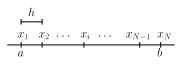
\includegraphics{./cap_pvc/pics/malha_uniforme/malha_uniforme}
  \caption{Malha uniforme de $N$ pontos em um intervalo $[a, b]$.}
  \label{fig:malha_uniforme}
\end{figure}

{\bf 1. Construção da malha.} A malha consiste em uma representação discreta do domínio $[a, b]$. Como veremos, sua construção tem impacto direto nas próximas etapas do método. Aqui, vamos construir a malha mais simples possível, aquela que consiste de $N$ pontos igualmente espaçados, isto é, a chamada \emph{malha uniforme}\index{malha uniforme}.

Para tanto, seja $N\in\mathbb{N}$ dado e, então, tomamos o seguinte conjunto discreto $\mathcal{P}_N = \{x_1, x_2, \dotsc, x_N\}$ (a malha), onde
\begin{equation*}
  x_i = a + (i-1)h,\quad i=1, 2, \dotsc, N,
\end{equation*}
com
\begin{equation*}
  h:=\frac{b-a}{N-1},
\end{equation*}
o qual é chamado de \emph{tamanho (ou passo) da malha}\index{tamanho da malha}\index{passo da malha} (veja a Figura~\ref{fig:malha_uniforme}).

{\bf 2. Construção do problema discreto.}\index{problema discreto} A segunda etapa consiste na discretização das equações, no nosso caso, das equações \eqref{eq:pvc1-eq}-\eqref{eq:pvc1-bc2}. 

Vamos começar pela Equação~\eqref{eq:pvc1-eq}. Em um ponto da malha $x_i$, $i = 2, 3, \dotsc, N-1$, temos
\begin{equation*}
  -u_{xx}(x_i) = f(x_i, u(x_i)).
\end{equation*}
Usando a fórmula de diferenças finitas central de ordem 2 para a segunda derivada, temos
\begin{equation*}
  -\left(\frac{u(x_i-h) - 2u(x_i) + u(x_i+h)}{h^2} + O(h^2)\right) = f(x_i, u(x_i)).
\end{equation*}
Rearranjando os termos, obtemos
\begin{equation*}
  -\frac{u(x_i-h) - 2u(x_i) + u(x_i+h)}{h^2} = f(x_i, u(x_i)) + O(h^2). 
\end{equation*}

Agora, denotando por $u_i$ a aproximação numérica de $u(x_i)$, a equação acima nos fornece
\begin{equation}\label{eq:pvc1-disc-eq}
\frac{1}{h^2}u_{i-1} - \frac{2}{h^2}u_i + \frac{1}{h^2}u_{i+1} = -f(x_i, u_i),
\end{equation}
para $i=2, 3, \dotsc, N-1$. Observamos que trata-se de um sistema de $N$ incógnitas, a saber $u_i$, e de $N-2$ equações, isto é, um sistema subdeterminado.

Para obtermos um sistema determinado, aplicamos as condições de contorno. Da condição de contorno dada na Equação~\eqref{eq:pvc1-bc1}, temos
\begin{equation}\label{eq:pvc1-disc-bc1}
  u(a) = u_a\Rightarrow u_1 = u_a.
\end{equation}
Analogamente, da condição de contorno dada na Equação~\eqref{eq:pvc1-bc1}, temos
\begin{equation}\label{eq:pvc1-disc-bc2}
  u(b) = u_b\Rightarrow u_N = u_b.
\end{equation}

Por fim, as equações \eqref{eq:pvc1-disc-bc2}, \eqref{eq:pvc1-disc-eq} e \eqref{eq:pvc1-disc-bc1} determinam o problema discreto associado
\begin{eqnarray}
  u_1 &=& u_a,\label{eq:pvc1-disc-eq1}\\
  \frac{1}{h^2}u_{i-1} - \frac{2}{h^2}u_i + \frac{1}{h^2}u_{i+1} &=& -f(x_i, u_i),\quad i=2, \dotsc, N-1,\label{eq:pvc1-disc-eqi}\\
  u_N &=& u_b.\label{eq:pvc1-disc-eqN}
\end{eqnarray}
Este é um sistema de equações de $N$ incógnitas e $N$ equações.

{\bf 3. Resolução do sistema discreto.} Esta etapa consiste em resolver o sistema discreto construído na etapa anterior. 

Para o PVC \eqref{eq:pvc1-eq}-\eqref{eq:pvc1-bc2}, construímos o problema discreto \eqref{eq:pvc1-disc-eq1}-\eqref{eq:pvc1-disc-eqN}. Este é um problema de $N$ equações e $N$ incógnitas. Observamos que se $f(x, u)$ é uma função linear, o sistema será linear e podemos resolver o sistema usando de técnicas numéricas para sistema lineares. Agora, se $f(x, u)$ é uma função não linear, podemos usar, por exemplo, do método de Newton para sistemas.

{\bf 4. Visualização e interpretação dos resultados.} A solução do problema discreto consiste dos valores $u_i$, isto é, de aproximações dos valores de $u$ nos pontos da malha. Para visualizarmos a solução podemos, por exemplo, construir o gráfico do conjunto de pontos $\{(x_i, u_i)\}$. Ainda, para obtermos aproximações da solução em outros pontos que não fazem parte da malha, podemos usar de técnicas de interpolação e/ou ajuste.

\begin{ex}\label{ex:pvc2}
  Use o método de diferenças finitas para resolver o seguinte problema de valor de contorno com condições de Dirichlet homogêneas:
  \begin{eqnarray}
    -u_{xx} &=& 100(x-1)^2,\quad 0 < x < 1,\label{eq:pvc2-eq}\\
    u(0) &=& 0,\label{eq:pvc2-bc1}\\
    u(1) &=& 0.\label{eq:pvc2-bc2}
  \end{eqnarray}
Use a fórmula de diferenças finitas central de ordem 2 para discretizar a derivada em uma malha uniforme de 11 pontos. Calcule, também, a solução analítica deste problema, faça um esboço das soluções numérica e analítica e compute o erro absoluto médio definido por
\begin{equation*}
  E := \frac{1}{N}\sum_{i=1}^N \left|u(x_i) - u_i\right|,
\end{equation*}
onde $x_i$ é o $i$-ésimo ponto da malha, $i=1, 2, \dotsc, N$ e $N$ é o número de pontos na mesma. Por fim, repita seus cálculos para uma malha com $101$ pontos. O que ocorre com o erro absoluto médio?
\end{ex}
\begin{sol} Vamos seguir as etapas conforme acima.

  {\bf 1. Construção da malha.} Tomando $N=11$, definimos os pontos da malha no domínio [0, 1] por:
  \begin{equation*}
    x_i = (i-1)h,\quad i=1, 2, \dotsc, N,
  \end{equation*}
com $h = 1/(N-1)$.

%%%%%%%%%%%%%%%%%%%%
% scilab
%%%%%%%%%%%%%%%%%%%%
\ifisscilab
No \verb+Scilab+, podemos construir a malha da seguinte forma:
\begin{verbatim}
a = 0
b = 1
N = 11
h = (b-a)/(N-1)
x = linspace(a,b,N)
\end{verbatim}
\fi
%%%%%%%%%%%%%%%%%%%%
%%%%%%%%%%%%%%%%%%%%
% octave
%%%%%%%%%%%%%%%%%%%%
\ifisoctave
No \verb+GNU Octave+, podemos construir a malha da seguinte forma:
\begin{verbatim}
a = 0
b = 1
N = 11
h = (b-a)/(N-1)
x = linspace(a,b,N)
\end{verbatim}
\fi
%%%%%%%%%%%%%%%%%%%%
%%%%%%%%%%%%%%%%%%%%
% python
%%%%%%%%%%%%%%%%%%%%
\ifispython
Em \verb+Python+, podemos construir a malha da seguinte forma:
\begin{verbatim}
a = 0
b = 1
N = 11
h = (b-a)/(N-1)
x = np.linspace(a,b,N)
\end{verbatim}
\fi
%%%%%%%%%%%%%%%%%%%%

{\bf 2. Construção do problema discreto.} Usando a fórmula de diferenças finitas central de ordem 2 para aproximar a derivada na Equação~\eqref{eq:pvc2-eq}, obtemos o seguinte sistema de equações:
\begin{equation*}
  - \frac{u_{i-1} - 2u_i + u_{i+1}}{h^2} = 100(x_i - 1)^2,\quad i = 2, \dotsc, N-1.
\end{equation*}
Completamos este sistema com as condições de contorno dadas nas equações~\eqref{eq:pvc2-bc1} e \eqref{eq:pvc2-bc2}, donde
\begin{equation*}
  u_1 = u_N = 0.
\end{equation*}
Ou seja, obtemos o seguinte problema discreto:
\begin{eqnarray}
  u_1 &=& 0,\label{eq:pvc2_disc_bc1}\\
  -\frac{1}{h^2}\left(u_{i+1} - 2u_i + u_{i+1}\right) &=& 100(x_i-1)^2,\quad i=2, \dotsc, N-1,\\
  u_N &=& 0.\label{eq:pvc2_disc_bc2}
\end{eqnarray}
Observamos que este é um sistema linear $N\times N$, o qual pode ser escrito na forma matricial $A\underline{u} = b$, cujos matriz de coeficientes é
\begin{equation*}
  A = 
  \begin{bmatrix}
    1 & 0 & 0 & 0 & 0 & \cdots & 0\\
    1 & -2 & 1 & 0 & 0 & \cdots & 0\\
    0 & 1 & -2 & 1 & 0 & \cdots & 0\\
    \vdots & \vdots & \vdots & \vdots & \vdots & \vdots & \vdots\\
    0 & 0 & 0 & 0 & 0 & \cdots & 1
  \end{bmatrix},
\end{equation*}
o vetor das incógnitas e o vetor dos termos constantes são
\begin{equation*}
  \underline{u} =
  \begin{bmatrix}
    u_1\\
    u_2\\
    u_3\\
    \vdots\\
    u_N
  \end{bmatrix}\quad\text{e}\quad
  b =
  \begin{bmatrix}
    0\\
    -100h^{2}(x_2-1)^2\\
    -100h^{2}(x_3-1)^2\\
    \vdots\\
    0
  \end{bmatrix}.
\end{equation*}

%%%%%%%%%%%%%%%%%%%%
% scilab
%%%%%%%%%%%%%%%%%%%%
\ifisscilab
No \verb+Scilab+, podemos construir o problema discreto a seguinte forma:
\begin{verbatim}
A = zeros(N,N)
b = zeros(N)

A(1,1) = 1
b(1) = 0
for i = 2:N-1
    A(i,i-1) = 1
    A(i,i) = -2
    A(i,i+1) = 1
    b(i) = -100 * h^2 * (x(i)-1)^2
end
A(N,N) = 1
b(N) = 0
\end{verbatim}
\fi
%%%%%%%%%%%%%%%%%%%%
%%%%%%%%%%%%%%%%%%%%
% octave
%%%%%%%%%%%%%%%%%%%%
\ifisoctave
No \verb+GNU Octave+, podemos construir o problema discreto a seguinte forma:
\begin{verbatim}
A = zeros(N,N)
b = zeros(N)

A(1,1) = 1
b(1) = 0
for i = 2:N-1
    A(i,i-1) = 1
    A(i,i) = -2
    A(i,i+1) = 1
    b(i) = -100 * h^2 * (x(i)-1)^2
end
A(N,N) = 1
b(N) = 0
\end{verbatim}
\fi
%%%%%%%%%%%%%%%%%%%%
%%%%%%%%%%%%%%%%%%%%
% python
%%%%%%%%%%%%%%%%%%%%
\ifispython
Em \verb+Python+, podemos construir o problema discreto a seguinte forma:
\begin{verbatim}
A = np.zeros((N,N))
b = np.zeros(N)

A[0,0] = 1
b[0] = 0
for i in np.arange(1,N-1):
    A[i,i-1] = 1
    A[i,i] = -2
    A[i,i+1] = 1
    b[i] = -100 * h**2 * (x[i]-1)**2
A[N-1,N-1] = 1
b[N-1] = 0
\end{verbatim}
\fi
%%%%%%%%%%%%%%%%%%%%

{\bf 3. Resolução do problema discreto.} Neste caso, o problema discreto consiste no sistema linear $A\underline{u} = b$ e, portanto, a solução é
\begin{equation}\label{eq:pvc2_numerica}
  \underline{u} = A^{-1}b.
\end{equation}

%%%%%%%%%%%%%%%%%%%%
% scilab
%%%%%%%%%%%%%%%%%%%%
\ifisscilab
No \verb+Scilab+, podemos computar a solução do sistema $A\underline{u} = b$ com:
\begin{verbatim}
u = A\b
\end{verbatim}
\fi
%%%%%%%%%%%%%%%%%%%%
%%%%%%%%%%%%%%%%%%%%
% octave
%%%%%%%%%%%%%%%%%%%%
\ifisoctave
No \verb+GNU Octave+, podemos computar a solução do sistema $A\underline{u} = b$ com:
\begin{verbatim}
u = A\b
\end{verbatim}
\fi
%%%%%%%%%%%%%%%%%%%%
%%%%%%%%%%%%%%%%%%%%
% python
%%%%%%%%%%%%%%%%%%%%
\ifispython
Em \verb+Python+, podemos computar a solução do sistema $A\underline{u} = b$ com:
\begin{verbatim}
u = np.linalg.solve(A,b)
\end{verbatim}
\fi
%%%%%%%%%%%%%%%%%%%%

\begin{figure}
  \centering
  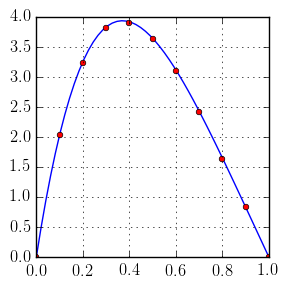
\includegraphics{./cap_pvc/pics/ex_pvc2/ex_pvc2}
  \caption{Esboço dos gráficos das soluções analítica (linha) e numérica (pontos) do PVC dado no Exemplo~\ref{ex:pvc2}.}
  \label{fig:ex_pvc2}
\end{figure}

{\bf 4. Visualização e interpretação dos resultados.} Tendo resolvido o problema discreto $A\underline{u} = b$, obtemos os valores da solução numérico de $u$ nos pontos da malha, isto é, obtivemos o conjunto de pontos $\{(x_i, u_i)\}_{i=1}^N$. Neste exemplo, queremos comparar a solução numérica com a solução analítica.

A solução analítica pode ser obtida por integração. Temos:
\begin{equation*}
  \begin{split}
    -u_{xx} = 100(x-1)^2 &\Rightarrow -u_x + c_1 = 100\frac{(x-1)^3}{3}\\
    \Rightarrow -u + c_2x + c_1 = 100\frac{(x-1)^4}{12},
  \end{split}
\end{equation*}
ou seja, $\displaystyle u(x) = - \frac{(x-1)^4}{12} + c_2x + c_1$. As constantes são determinadas pelas condições de contorno dadas pelas equações~\eqref{eq:pvc2-bc1} e \eqref{eq:pvc2-bc2}, isto é:
\begin{equation*}
  \begin{split}
    u(0) = 0 &\Rightarrow c_1 = \frac{100}{12},\\
    u(1) = 0 &\Rightarrow c_2 = -\frac{100}{12}.
  \end{split}
\end{equation*}
Portanto, a solução analítica é:
\begin{equation}\label{eq:pvc2_analitica}
  u(x) = -100\frac{(x-1)^4}{12} - 100\frac{x}{12} + \frac{100}{12}
\end{equation}

A Figura~\ref{fig:ex_pvc2} mostra o esboço dos gráficos das soluções analítica \eqref{eq:pvc2_analitica} e a da solução numérica \eqref{eq:pvc2_numerica}.

%%%%%%%%%%%%%%%%%%%%
% scilab
%%%%%%%%%%%%%%%%%%%%
\ifisscilab
No \verb+Scilab+, podemos fazer o esboço das soluções analítica e numérica da seguinte forma:
\begin{verbatim}
//def. sol. analitica
deff('y = ue(x)','y = -100.0*(x-1).^4/12 - 100*x/12 + 100.0/12')

//grafico
xx = linspace(0,1)
yy = ue(xx)

plot(x,u,'ro',xx,yy,'b-')
\end{verbatim}
\fi
%%%%%%%%%%%%%%%%%%%%
%%%%%%%%%%%%%%%%%%%%
% octave
%%%%%%%%%%%%%%%%%%%%
\ifisoctave
No \verb+GNU Octave+, podemos fazer o esboço das soluções analítica e numérica da seguinte forma:
\begin{verbatim}
#def. sol. analitica
ue = inline("-100.0*(x-1).^4/12 - 100*x/12 + 100.0/12")

#grafico
xx = linspace(0,1)
yy = ue(xx)

plot(x,u,'ro',xx,yy,'b-')
\end{verbatim}
\fi
%%%%%%%%%%%%%%%%%%%%
%%%%%%%%%%%%%%%%%%%%
% python
%%%%%%%%%%%%%%%%%%%%
\ifispython
Em \verb+Python+, podemos fazer o esboço das soluções analítica e numérica da seguinte forma:
\begin{verbatim}
#def. sol. analitica
def ue(x):
    return -100.0*(x-1)**4/12 - 100*x/12 + 100.0/12

#grafico
xx = np.linspace(0,1)
yy = np.zeros(50)
for i,xxi in enumerate(xx):
    yy[i] = ue(xxi)

plt.plot(x',u,'ro',xx,yy,'b-')
plt.show()
\end{verbatim}
\fi
%%%%%%%%%%%%%%%%%%%%

\begin{table}
  \centering
  \caption{Erro absoluto médio das soluções numéricas com $N=11$ e $N=101$ do PVC dado no Exemplo~\ref{ex:pvc2}.}
  \begin{tabular}{ll|c}
    $N$ & $h$ & $E$\\\hline
    11 & 0,1 & $1,3\times 10^{-2}$\\
    101 & 0,01 & $1,4\times 10^{-4}$
  \end{tabular}
  \label{tab:pvc2_erro}
\end{table}

Por fim, computamos o erro absoluto médio das soluções numéricas com $N=11$ e $N=101$. A Tabela~\ref{tab:pvc2_erro} mostra os resultados obtidos. Observamos, que ao diminuirmos $10$ vezes o tamanho do passo $h$, o erro absoluto médio diminui aproximadamente $100$ vezes. Este resultado é esperado, pois o problema discreto \eqref{eq:pvc2_disc_bc1}-\eqref{eq:pvc2_disc_bc2} aproxima o problema contínuo \eqref{eq:pvc2-eq}-\eqref{eq:pvc2-bc2} com erro de truncamento de ordem $h^2$. Verifique!

%%%%%%%%%%%%%%%%%%%%
% scilab
%%%%%%%%%%%%%%%%%%%%
\ifisscilab
No \verb+Scilab+, podemos computar o erro absoluto médio da seguinte forma:
\begin{verbatim}
E = sum(abs(ue(x)' - u))/N
\end{verbatim}
\fi
%%%%%%%%%%%%%%%%%%%%
%%%%%%%%%%%%%%%%%%%%
% octave
%%%%%%%%%%%%%%%%%%%%
\ifisoctave
No \verb+GNU Octave+, podemos computar o erro absoluto médio da seguinte forma:
\begin{verbatim}
E = sum(abs(ue(x)' - u))/N
\end{verbatim}
\fi
%%%%%%%%%%%%%%%%%%%%
%%%%%%%%%%%%%%%%%%%%
% python
%%%%%%%%%%%%%%%%%%%%
\ifispython
Em \verb+Python+, podemos computar o erro absoluto médio da seguinte forma:
\begin{verbatim}
E = 0
for i,xi in enumerate(x):
    E += np.abs(ue(xi) - u[i])
E /= N
\end{verbatim}
\fi
%%%%%%%%%%%%%%%%%%%%
\end{sol}

\subsection*{Exercícios resolvidos}

\begin{exeresol}\label{exeresol:pvc_linear} Use o método de diferenças finitas para resolver o seguinte problema de valor de contorno:
  \begin{eqnarray}
    -u_{xx} + u  &=& e^{-x},\quad 0<x<1,\\
    u(0,5) &=& 1,\\
    u(1,5) &=& 2.
  \end{eqnarray}
Para tanto, use a fórmula de diferenças finitas central de ordem 2 para discretizar a derivada em uma malha uniforme com passo $h=0,1$. Faça, então, um esboço do gráfico da solução computada.
\end{exeresol}
\begin{resol}
O passo $h$ é uma malha uniforme com $N$ pontos no domínio $[0,5, 1,5]$ satisfaz:
\begin{equation*}
  h = \frac{(b-a)}{N-1} \Rightarrow N = \frac{(b-a)}{h} + 1.
\end{equation*}
Ou seja, a malha deve conter $N = 11$ pontos igualmente espaçados. Denotamos os pontos na malha por $x_i$, onde $x_i = 0,5 + (i-1)h$.

\begin{table}
  \centering
  \begin{tabular}{cc|cc}
    $x$ & $u$ & $x$ & $u$\\\hline
0.50 & 1.000000 & 1.00 & 1.643900 \\
0.60 & 1.143722 & 1.10 & 1.745332 \\
0.70 & 1.280661 & 1.20 & 1.834176 \\
0.80 & 1.410269 & 1.30 & 1.908160 \\
0.90 & 1.531724 & 1.40 & 1.964534 \\
1.00 & 1.643900 & 1.50 & 2.000000 \\\hline
  \end{tabular}
  \caption{Solução numérica do Exercício~\ref{exeresol:pvc_linear}.}
  \label{tab:exeresol_pvc_linear}
\end{table}

Agora, a equação diferencial dada no $i$-ésimo ponto da malha é:
\begin{equation*}
  -u_{xx}(x_i) + u(x_i) = e^{x_i},\quad i = 2, 3, \dotsc, N-1.
\end{equation*}
Denotando $u_i \approx u(x_i)$ e usando a fórmula de diferenças finitas central de ordem dois para a derivada $u_{xx}$, obtemos:
\begin{equation*}
  -\left(\frac{u_{i-1} - 2u_i + u_{i+1}}{h^2}\right) + u_i = e^{x_i},
\end{equation*}
para $i= 2, 3, \dotsc, N-1$. Rearranjando os termos e aplicando as condições de contorno, temos o problema discretizado como segue:
\begin{equation*}
  \begin{split}
    u_1 &= 1\\
    -u_{i-1} + (2 + h^2)u_i - u_{i+1} &= h^2e^{x_i},\quad i=2 ,\dotsc, N-1,\\
    u_N &= 2.
  \end{split}
\end{equation*}

\begin{figure}
  \centering
  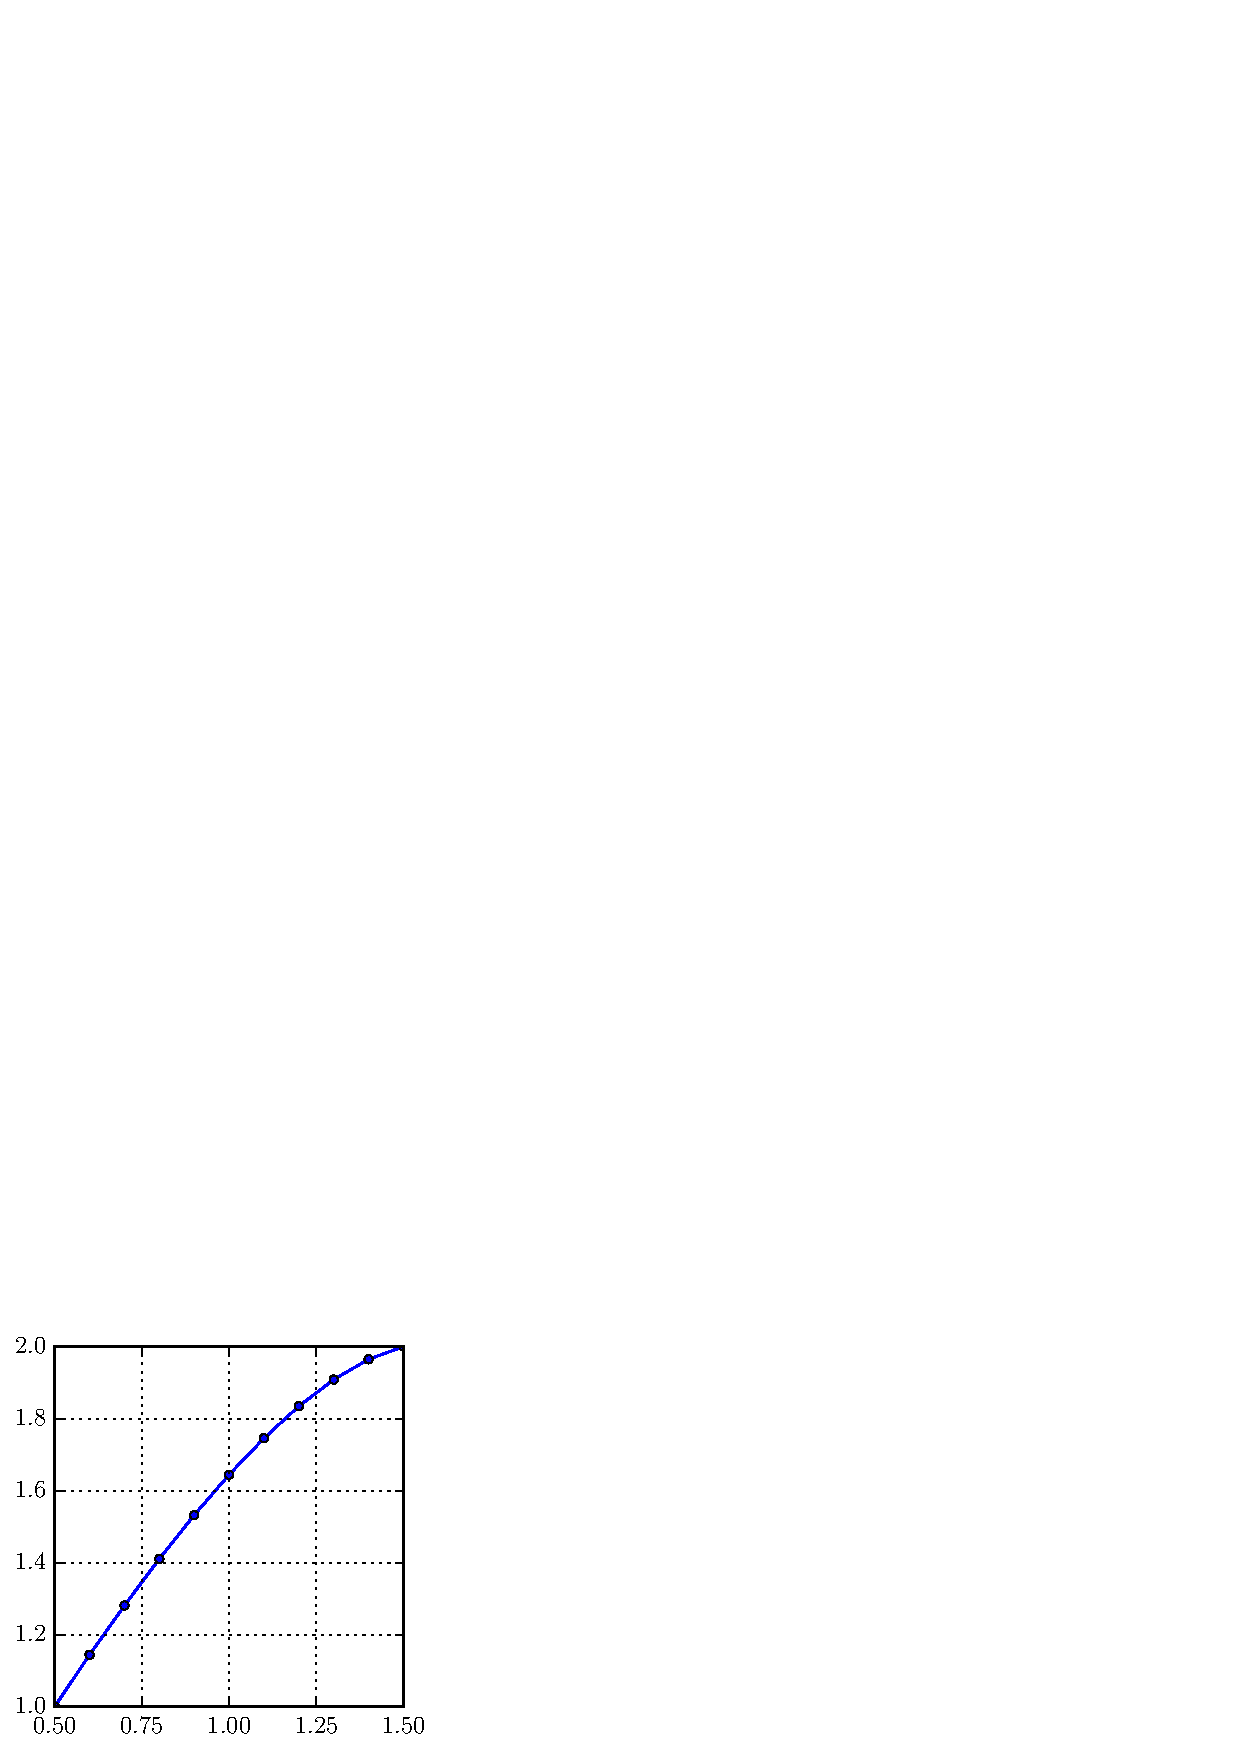
\includegraphics{./cap_pvc/pics/exeresol_pvc_linear/exeresol_pvc_linear}
  \caption{Esboço do gráfico da solução numérica do Exercício~\ref{exeresol:pvc_linear}.}
  \label{fig:exeresol_pvc_linear}
\end{figure}

O problema discreto obtido é um sistema linear $N\times N$. Resolvendo este sistema, obtemos a solução discreta apresentada na Tabela~\ref{tab:exeresol_pvc_linear}. A Figura~\ref{fig:exeresol_pvc_linear} mostra um esboço do gráfico da solução computada.

%%%%%%%%%%%%%%%%%%%%
% scilab
%%%%%%%%%%%%%%%%%%%%
\ifisscilab
No \verb+Scilab+, podemos computar a solução numérica e graficá-la com o seguinte código:
\begin{verbatim}
//malha
a = 0.5
b = 1.5
N = 11
h = (b-a)/(N-1)
x = linspace(a,b,N)'

//sistema
A = zeros(N,N)
b = zeros(N,1)

A(1,1) = 1
b(1) = 1
for i = 2:N-1
    A(i,i-1) = -1
    A(i,i) = 2 + h^2
    A(i,i+1) = -1
    b(i) = h^2 * exp(x(i))
end
A(N,N) = 1
b(N) = 2

//solucao
u = A\b

//grafico
plot(x,u,'b-o')
\end{verbatim}
\fi
%%%%%%%%%%%%%%%%%%%%
%%%%%%%%%%%%%%%%%%%%
% octave
%%%%%%%%%%%%%%%%%%%%
\ifisoctave
No \verb+GNU Octave+, podemos computar a solução numérica e graficá-la com o seguinte código:
\begin{verbatim}
#malha
a = 0.5
b = 1.5
N = 11
h = (b-a)/(N-1)
x = linspace(a,b,N)'

#sistema
A = zeros(N,N)
b = zeros(N,1)

A(1,1) = 1
b(1) = 1
for i = 2:N-1
    A(i,i-1) = -1
    A(i,i) = 2 + h^2
    A(i,i+1) = -1
    b(i) = h^2 * exp(x(i))
endfor
A(N,N) = 1
b(N) = 2

#solucao
u = A\b

#grafico
plot(x,u,'b-o')
\end{verbatim}
\fi
%%%%%%%%%%%%%%%%%%%%
%%%%%%%%%%%%%%%%%%%%
% python
%%%%%%%%%%%%%%%%%%%%
\ifispython
Em \verb+Python+, podemos computar a solução numérica e graficá-la com o seguinte código:
\begin{verbatim}
#malha
a = 0.5
b = 1.5
N = 11
h = (b-a)/(N-1)
x = np.linspace(a,b,N)

#sistema
A = np.zeros((N,N))
b = np.zeros(N)

A[0,0] = 1
b[0] = 1
for i in np.arange(1,N-1):
    A[i,i-1] = -1
    A[i,i] = 2 + h**2
    A[i,i+1] = -1
    b[i] = h**2 * np.exp(x[i])
A[N-1,N-1] = 1
b[N-1] = 2

#solucao
u = np.linalg.solve(A,b)

#grafico
plt.plot(x,u,'b-o')
plt.show()
\end{verbatim}
\fi
%%%%%%%%%%%%%%%%%%%%
\end{resol}

\subsection*{Exercícios}

\begin{exer}
 Considere o seguinte problema de valor de contorno para a equação de calor no estado estacionário:
$$\left\{\begin{array}{l}-u_{xx}=32,~~ 0<x<1.\\
u(0)=5\\
u(1)=10\end{array}
\right.
$$

Defina $u_j=u(x_j)$ onde $x_j={(j-1)}{h}$ e $j=1,\ldots,5$. Aproxime a derivada segunda por um esquema de segunda ordem e transforme a equação diferencial em um sistema de equações lineares. Escreva este sistema linear na forma matricial e resolva-o. Faça o mesmo com o dobro de subintervalos, isto é, com malha de 9 pontos. 
\end{exer}
\begin{resp}
 $$\left[
  \begin{array}{ccccc}
         1 & 0& 0& 0& 0\\
         -1 & 2 & -1 &0&0\\
         0&-1 & 2 & -1 &0\\
         0&0&-1 & 2 & -1 \\
         0 & 0& 0& 0& 1\\
        \end{array}
\right]
\left[
  \begin{array}{c}
     u_1\\ u_2\\u_3\\u_4 \\ u_5
   \end{array}
\right]
=
\left[
  \begin{array}{c}
     5\\ 2\\2\\2 \\ 10
   \end{array}
\right]
$$


Solução:  [5, 9.25, 11.5, 11.75, 10]    

$$\left[
  \begin{array}{ccccccccc}
         1 & 0& 0& 0& 0& 0& 0& 0& 0\\
         -1 & 2 & -1 &0&0& 0& 0& 0& 0\\
         0&-1 & 2 & -1 &0& 0& 0& 0& 0\\
         0&0&-1 & 2 & -1 & 0& 0& 0& 0\\
         0&0&0&-1 & 2 & -1 & 0& 0& 0\\
         0&0&0&0&-1 & 2 & -1 & 0& 0\\
         0&0&0&0&0&-1 & 2 & -1 & 0\\
         0&0&0&0&0&0&-1 & 2 & -1\\
         0 & 0& 0& 0& 0& 0& 0& 0& 1\\
        \end{array}
\right]
\left[
  \begin{array}{c}
     u_1\\ u_2\\u_3\\u_4 \\u_5\\ u_6\\u_7\\u_8\\u_9
   \end{array}
\right]
=
\left[
  \begin{array}{c}
     5\\ 0.5\\0.5\\0.5\\ 0.5\\0.5\\0.5\\0.5 \\ 10
   \end{array}
\right]
$$

Solução:  $[5, 7.375, 9.25, 10.625, 11.5, 11.875, 11.75, 1.125, 10]$
\end{resp}


\begin{exer} Considere o seguinte problema de valor de contorno para a equação de calor no estado estacionário:
$$\left\{\begin{array}{l}-u_{xx}=200e^{-(x-1)^2},~~ 0<x<2.\\
u(0)=120\\
u(2)=100\end{array}
\right.
$$
Defina $u_j=u(x_j)$ onde $x_j={(j-1)}{h}$ e $j=1,\ldots,21$. Aproxime a derivada segunda por um esquema de segunda ordem e transforme a equação diferencial em um sistema de equações lineares. Resolva o sistema linear obtido.
\end{exer}
\begin{resp}
120.    133.56    146.22    157.83    168.22    177.21    184.65    190.38    194.28    196.26    196.26    194.26    190.28    184.38    176.65    167.21  156.22    143.83    130.22    115.56    100.    
\end{resp}

\begin{exer} Considere o seguinte problema de valor de contorno para a equação de calor no estado estacionário:
$$\left\{\begin{array}{l}-u_{xx}=200e^{-(x-1)^2},~~ 0<x<2.\\
u'(0)=0\\
u(2)=100\end{array}
\right.
$$
Defina $u_j=u(x_j)$ onde $x_j={(j-1)}{h}$ e $j=1,\ldots,21$. Aproxime a derivada segunda por um esquema de segunda ordem, a derivada primeira na fronteira por um esquema de primeira ordem e transforme a equação diferencial em um sistema de equações lineares. Resolva o sistema linear obtido.
\end{exer}
\begin{resp}
391.13    391.13    390.24    388.29    385.12    380.56    374.44    366.61    356.95    345.38    331.82    316.27    298.73    279.27    257.99    234.99    210.45    184.5    157.34    129.11    100.    
\end{resp}


\begin{exer} Considere o seguinte problema de valor de contorno para a equação de calor no estado estacionário com um termo não linear de radiação:
$$\left\{\begin{array}{l}-u_{xx}=100- \frac{u^4}{10000},~~ 0<x<2.\\
u(0)=0\\
u(2)=10\end{array}
\right.
$$
Defina $u_j=u(x_j)$ onde $x_j={(j-1)}{h}$ e $j=1,\ldots,21$. Aproxime a derivada segunda por um esquema de segunda ordem e transforme a equação diferencial em um sistema de equações não lineares. Resolva o sistema  obtido. Expresse  a solução com dois algarismos depois do separador decimal. Dica: Veja problema 38 da lista 2, seção de sistemas não lineares.
\end{exer}
\begin{resp}
0.,    6.57,    12.14,    16.73,    20.4,    23.24,    25.38,    26.93 ,   28,    28.7,    29.06,    29.15,    28.95,    28.46, 27.62 ,   26.36,    24.59,    22.18,    19.02,    14.98,    10.    
\end{resp}

\begin{exer} Considere o seguinte problema de valor de contorno para a equação de calor no estado estacionário com um termo não linear de radiação e um termo de convecção:
$$\left\{\begin{array}{l}-u_{xx}+3u_x=100- \frac{u^4}{10000},~~ 0<x<2.\\
u'(0)=0\\
u(2)=10\end{array}
\right.
$$
Defina $u_j=u(x_j)$ onde $x_j={(j-1)}{h}$ e $j=1,\ldots,21$. Aproxime a derivada segunda por um esquema de segunda ordem, a derivada primeira na fronteira por um esquema de primeira ordem, a derivada primeira no interior por um esquema de segunda ordem e transforme a equação diferencial em um sistema de equações não lineares. Resolva o sistema  obtido.
\end{exer}
\begin{resp}
$u(0)=31.62$, $u(1)=31,50$, $u(1,9)=18,17$.    
\end{resp}

\begin{exer} Considere o seguinte problema de valor de contorno:
$$\left\{\begin{array}{l}-u''+2u'=e^{-x}- \frac{u^2}{100},~~ 1<x<4.\\
u'(1)+u(1)=2\\
u'(4)=-1\end{array}
\right.
$$
Defina $u_j=u(x_j)$ onde $x_j=1+{(j-1)}{h}$ e $j=1,\ldots,101$. Aproxime a derivada segunda por um esquema de segunda ordem, a derivada primeira na fronteira por um esquema de primeira ordem, a derivada primeira no interior por um esquema de segunda ordem e transforme a equação diferencial em um sistema de equações não lineares. Resolva o sistema  obtido.
\end{exer}
\begin{resp}
$u(1)=1,900362$, $u(2,5)=1.943681$, $u(4)=1,456517$.    
\end{resp}

%\end{document} 
